\documentclass[11pt,oneside]{article}

\usepackage[a4paper,margin=27mm,headheight=15pt]{geometry}
\usepackage[T1]{fontenc}
\usepackage[utf8]{inputenc}
\IfFileExists{libertinus.sty}{\usepackage{libertinus}}{\usepackage{lmodern}}
\usepackage{microtype}
\usepackage{amsmath,amssymb,amsthm,mathtools,mathrsfs}
\usepackage{bm}
\usepackage{booktabs,longtable,array,tabularx,multirow}
\usepackage[table]{xcolor}
\usepackage{tikz}
\usepackage{enumitem}
\usepackage{fancyhdr}
\usepackage{titlesec}
\usepackage{listings}
\usepackage{xurl}
\usepackage{hyperref}
\usepackage[nameinlink,noabbrev]{cleveref}

\definecolor{linkblue}{RGB}{25,75,135}
\definecolor{deepteal}{RGB}{25,96,101}
\definecolor{softolive}{RGB}{120,128,68}
\definecolor{shadegray}{RGB}{246,247,249}
\definecolor{rulegray}{RGB}{195,201,208}
\definecolor{rootcell}{RGB}{78,111,86}
\definecolor{lightroot}{RGB}{225,232,222}

\hypersetup{
  colorlinks=true,
  linkcolor=linkblue,
  citecolor=linkblue,
  urlcolor=linkblue,
  pdftitle={Diagonal Polynomial Laws in Odd Iterated Thue--Morse Summation},
  pdfauthor={Vladimir Reshetnikov},
  pdfsubject={Riordan arrays, Thue--Morse prefix sums, diagonal polynomials, Fabius approximants},
  pdfkeywords={Thue-Morse, Fabius function, Riordan array, Sheffer polynomial, Bell polynomial, repeated summation}
}

\pagestyle{fancy}
\fancyhf{}
\fancyhead[L]{\small Thue--Morse diagonal polynomials}
\fancyhead[R]{\small\nouppercase{\leftmark}}
\fancyfoot[C]{\thepage}
\renewcommand{\headrulewidth}{0.4pt}

\titleformat{\section}{\Large\bfseries}{\thesection}{0.7em}{}
\titleformat{\subsection}{\large\bfseries}{\thesubsection}{0.7em}{}
\titleformat{\subsubsection}{\normalsize\bfseries}{\thesubsubsection}{0.7em}{}
\setcounter{secnumdepth}{3}
\setcounter{tocdepth}{2}
\setlist[itemize]{leftmargin=2em,itemsep=0.25em,topsep=0.4em}
\setlist[enumerate]{leftmargin=2.3em,itemsep=0.25em,topsep=0.4em}
\setlength{\emergencystretch}{2.5em}

\newtheorem{theorem}{Theorem}[section]
\newtheorem{proposition}[theorem]{Proposition}
\newtheorem{lemma}[theorem]{Lemma}
\newtheorem{corollary}[theorem]{Corollary}
\newtheorem{conjecture}[theorem]{Conjecture}
\theoremstyle{definition}
\newtheorem{definition}[theorem]{Definition}
\newtheorem{algorithm}[theorem]{Algorithm}
\newtheorem{example}[theorem]{Example}
\theoremstyle{remark}
\newtheorem{remark}[theorem]{Remark}
\newtheorem{warning}[theorem]{Warning}

\newcommand{\N}{\mathbb N}
\newcommand{\Z}{\mathbb Z}
\newcommand{\Q}{\mathbb Q}
\newcommand{\R}{\mathbb R}
\newcommand{\eps}{\varepsilon}
\newcommand{\Diag}{D}
\newcommand{\Prefix}{\mathcal P}
\newcommand{\TM}{\mathcal T}
\newcommand{\coeff}[2]{[z^{#1}]\,#2}
\newcommand{\vtwo}{\nu_{2}}
\newcommand{\bitsum}{s_{2}}
\newcommand{\rising}[2]{#1^{\overline{#2}}}
\newcommand{\falling}[2]{#1^{\underline{#2}}}
\newcommand{\dd}{\,\mathrm d}
\newcommand{\bigO}{\mathcal O}
\newcommand{\ind}{\mathbf 1}
\DeclareMathOperator{\popcount}{popcount}
\DeclareMathOperator{\ord}{ord}
\DeclareMathOperator{\lcm}{lcm}
\DeclareMathOperator{\sgn}{sgn}

\newenvironment{resultbox}{%
  \par\smallskip\noindent\begin{center}\begin{minipage}{0.94\textwidth}%
  \color{black}\hrule\vspace{0.65em}\small
}{%
  \vspace{0.65em}\hrule\end{minipage}\end{center}\smallskip
}

\lstdefinelanguage{Wolfram}{
  morekeywords={ClearAll,Module,With,If,And,Table,Sum,Product,Expand,Factor,
    Binomial,Floor,Quotient,QuotientRemainder,IntegerExponent,ThueMorse,
    Accumulate,Nest,CoefficientList,Take,Together,Numerator,Denominator,
    ConstantArray,OddQ,EvenQ,Range,Length,HoldForm,SetDelayed,True,False},
  sensitive=true,
  morecomment=[s]{(*}{*)},
  morestring=[b]"
}

\lstdefinestyle{code}{
  basicstyle=\ttfamily\small,
  backgroundcolor=\color{shadegray},
  frame=single,
  rulecolor=\color{rulegray},
  columns=fullflexible,
  keepspaces=true,
  showstringspaces=false,
  breaklines=true,
  breakatwhitespace=false,
  xleftmargin=0.7em,
  xrightmargin=0.7em,
  aboveskip=0.8em,
  belowskip=0.8em,
  tabsize=2
}

\title{\bfseries Diagonal Polynomial Laws in Odd Iterated\\
Thue--Morse Summation\\[0.35em]
\large Riordan-array structure, $2$-adic Bell recurrences, exact arithmetic,\\
and fast Wolfram Language evaluation}
\author{Vladimir Reshetnikov\\
\small ProveIt Fabius-function research program}
\date{3 September 2026}

\begin{document}
\maketitle

\begin{abstract}
Let $\eps_j=(-1)^{\bitsum(j)}$ be the signed Thue--Morse sequence and let
$S^{(r)}=\Prefix^r\eps$ denote $r$ inclusive prefix summations.  The table in
the question is, after making its shift explicit,
\[
 s(n,k)=S^{(2n+1)}(k-n-1)\qquad (k\ge n+1),
\]
with $s(n,k)=0$ for $k\le n$.  For a fixed diagonal offset $m$ define
$\Diag_m(n)=s(n,n+1+m)$.  The principal result is the formal generating
identity
\[
 \sum_{m\ge0}\Diag_m(x)z^m
   =\frac{\TM(z^2)}{(1-z)^{2x}},
 \qquad
 \TM(z)=\prod_{j\ge0}(1-z^{2^j})
       =\sum_{q\ge0}\eps_qz^q,
\]
which yields the exact polynomial formula
\[
 \Diag_m(x)=\sum_{q=0}^{\lfloor m/2\rfloor}
   \eps_q\binom{2x+m-2q-1}{m-2q}.
\]
Thus the $m$th diagonal is a degree-$m$ polynomial with leading coefficient
$2^m/m!$.  After shifting the column index, the complete two-dimensional
table is the unit lower-triangular Riordan array
\[
 \left(\TM(z^2),\frac{z}{(1-z)^2}\right).
\]
This observation is developed into a general subdiagonal theorem for proper
Riordan arrays.

The logarithm of the diagonal generating function has the unusually simple
$2$-adic cumulants
\[
 \lambda_r(x)=2x+2-2^{\vtwo(r)+1},
\]
so the polynomials satisfy a Newton--Bell recurrence, complete Bell-polynomial
and partition formulas, and a determinant formula.  They also form a Sheffer
sequence for the half-step difference operator:
\[
 \Diag_m(x)-\Diag_m\!\left(x-\tfrac12\right)=\Diag_{m-1}(x).
\]
The arithmetic is exact: $m!\Diag_m(x)/2^{\lceil m/2\rceil}$ is a primitive
integer polynomial, giving the exact common denominator of every diagonal.
Every rational zero is an integer or a half-integer.  All nonnegative rational
zeros are classified by a dyadic residue condition, which explains the
visible factors $x$, $2x-1$, $x-1$, and their higher analogues.  Negative
half-grid values have a finite binomial--Thue--Morse formula.

Finally, the row factorization into finite geometric products proves the
block repetition, reflection, complement, plateau, and zero-run rules used by
the supplied Wolfram Language program.  A new signed-prefix-moment recursion
then evaluates an arbitrary table entry in $O(n^2\log m)$ exact arithmetic
operations, where $m=k-n-1$, rather than summing $O(m)$ terms.  Complete
Wolfram Language and Python implementations accompany the article.
\end{abstract}

\tableofcontents
\newpage

\section{Scope, conventions, and repository context}
\label{sec:scope}

The \texttt{ProveIt} Fabius-function development contains an early note on
iterated summation of signed Thue--Morse prefixes and a later Lean development
that formalizes the exact convolution, generating-series, zero-run, and
approximation statements \cite{proveit-early,proveit-prefix,proveit-approx}.
It also contains a machine-checked audit that refutes several unrelated
asymptotic and normalization claims in the early note
\cite{proveit-audit}.  The present article uses only the exact discrete
structure.  In particular, none of the refuted proxy or error estimates is
used here.

The diagonal identities, Riordan-array interpretation, $2$-adic Bell
recurrence, primitive normalization, rational-root restriction, and fast
prefix-moment evaluator below are derived directly from the formal power
series of the table.  They should therefore be read as an algebraic companion
to the repository's analytic Fabius approximation theory.  No claim of
literature priority is intended beyond this repository-level comparison.

Throughout,
\[
 \N=\{0,1,2,\ldots\},\qquad
 \eps_j=(-1)^{\bitsum(j)}=(-1)^{\popcount(j)},
\]
where $\bitsum(j)$ is the sum of the binary digits of $j$.  We use the
standard identities
\begin{equation}
 \eps_{2j}=\eps_j,
 \qquad
 \eps_{2j+1}=-\eps_j.
 \label{eq:tm-doubling}
\end{equation}
All generating-function identities are identities in a formal power-series
ring over $\Q$ unless an analytic domain is stated explicitly.  Consequently
there are no convergence issues in coefficient extraction.

\begin{resultbox}
\textbf{Indexing guide.}
The row parameter $n$ in the code is not the number of prefix summations.
Row $n$ contains the $(2n+1)$-fold inclusive prefix sum, shifted right by
$n+1$ columns.  The natural diagonal coordinate is
\[
 m=k-n-1.
\]
The polynomial $\Diag_m(x)$ describes the line $k=n+1+m$; its value at the
integer $x=n$ is exactly the table entry on that line.
\end{resultbox}

\section{From inclusive prefix sums to the table}
\label{sec:prefix}

\subsection{The prefix operator and its convolution kernel}

For a sequence $a=(a_0,a_1,\ldots)$ define the inclusive prefix operator
\[
 (\Prefix a)_r=\sum_{j=0}^{r}a_j,
 \qquad r\in\N.
\]
Let $S^{(0)}_r=\eps_r$ and $S^{(\ell)}=\Prefix^\ell\eps$ for
$\ell\ge1$.

\begin{proposition}[Iterated-prefix convolution]
\label{prop:prefix-convolution}
For $\ell\ge1$ and $r\ge0$,
\begin{equation}
 S^{(\ell)}_r
   =\sum_{j=0}^{r}
      \binom{r-j+\ell-1}{\ell-1}\eps_j.
 \label{eq:prefix-convolution}
\end{equation}
Equivalently,
\begin{equation}
 \sum_{r\ge0}S^{(\ell)}_rz^r
   =\frac{\TM(z)}{(1-z)^\ell},
 \qquad
 \TM(z):=\sum_{j\ge0}\eps_jz^j.
 \label{eq:prefix-ogf}
\end{equation}
\end{proposition}

\begin{proof}
One prefix summation multiplies an ordinary generating function by
$(1-z)^{-1}$:
\[
 \sum_{r\ge0}\left(\sum_{j=0}^{r}a_j\right)z^r
 =\sum_{j\ge0}a_jz^j\sum_{h\ge0}z^h
 =\frac{1}{1-z}\sum_{j\ge0}a_jz^j.
\]
Iterating gives \eqref{eq:prefix-ogf}.  The coefficient of $z^{r-j}$ in
$(1-z)^{-\ell}$ is
$\binom{r-j+\ell-1}{\ell-1}$, which gives
\eqref{eq:prefix-convolution}.
\end{proof}

The signed Thue--Morse generating series has the classical product
\begin{equation}
 \TM(z)=\prod_{j=0}^{\infty}(1-z^{2^j}).
 \label{eq:tm-product}
\end{equation}
Indeed, choosing either $1$ or $-z^{2^j}$ from each factor records the binary
expansion of the exponent, with sign $(-1)^{\bitsum(j)}$.  Separating the
first factor gives the particularly useful functional identity
\begin{equation}
 \TM(z)=(1-z)\TM(z^2).
 \label{eq:T-functional}
\end{equation}
The product and its many consequences are standard in the theory of the
Prouhet--Thue--Morse sequence \cite{allouche-shallit-1999,automatic-sequences}.

\subsection{Exact identification of the code's row and column indices}

\begin{definition}[The shifted odd-prefix table]
\label{def:s-table}
For $n,k\in\N$ define
\begin{equation}
 s(n,k)=
 \begin{cases}
  0,&k\le n,\\[0.25em]
  S^{(2n+1)}_{k-n-1},&k\ge n+1.
 \end{cases}
 \label{eq:s-prefix-identification}
\end{equation}
\end{definition}

\begin{proposition}[Agreement with the twofold-summation recurrence]
\label{prop:user-recurrence}
For $n\ge1$ and $k\ge0$,
\begin{equation}
 s(n,k)=\sum_{j=0}^{k-1}(k-j)s(n-1,j),
 \label{eq:user-recurrence}
\end{equation}
where an empty sum is zero.
\end{proposition}

\begin{proof}
For any sequence $a$,
\[
 (\Prefix^2a)_N
   =\sum_{t=0}^{N}(N-t+1)a_t.
\]
Take $a_t=S^{(2n-1)}_t$ and $N=k-n-1$.  In the sum on the right side of
\eqref{eq:user-recurrence}, all terms with $j\le n-1$ vanish by definition.
Writing $t=j-n$ in the remaining terms gives
\[
 \sum_{j=n}^{k-1}(k-j)S^{(2n-1)}_{j-n}
 =\sum_{t=0}^{k-n-1}(k-n-t)S^{(2n-1)}_t
 =S^{(2n+1)}_{k-n-1}.
\]
This is $s(n,k)$ by \eqref{eq:s-prefix-identification}.
\end{proof}

The convolution formula now gives a direct expression for every table entry.

\begin{corollary}[Single-sum formula for the complete table]
\label{cor:s-direct}
For $k\ge n+1$,
\begin{equation}
 s(n,k)=\sum_{j=0}^{k-n-1}
   \binom{k+n-1-j}{2n}\eps_j.
 \label{eq:s-direct}
\end{equation}
\end{corollary}

\begin{proof}
Apply \cref{prop:prefix-convolution} with $\ell=2n+1$ and
$r=k-n-1$.
\end{proof}

\subsection{Row generating functions}

Let
\[
 G_n(z)=\sum_{k\ge0}s(n,k)z^k.
\]
The shift by $n+1$, \eqref{eq:prefix-ogf}, and
\eqref{eq:T-functional} give two equivalent forms:
\begin{align}
 G_n(z)
 &=z^{n+1}\frac{\TM(z)}{(1-z)^{2n+1}}
 \label{eq:row-gf-first}\\
 &=z^{n+1}\frac{\TM(z^2)}{(1-z)^{2n}}.
 \label{eq:row-gf}
\end{align}
In particular,
\begin{equation}
 \frac{G_n(z)}{G_{n-1}(z)}=\frac{z}{(1-z)^2}
 \qquad(n\ge1).
 \label{eq:row-ratio}
\end{equation}
The cumulative recurrence in the original code is therefore the integrated
form of a local second-difference law.

\begin{corollary}[Local discrete equation]
\label{cor:local-pde}
With the convention $s(n,k)=0$ for $k<0$, one has, for $n\ge1$,
\begin{equation}
 s(n,k)-2s(n,k-1)+s(n,k-2)=s(n-1,k-1).
 \label{eq:local-pde}
\end{equation}
\end{corollary}

\begin{proof}
Multiply \eqref{eq:row-ratio} by $(1-z)^2$ and compare coefficients of
$z^k$.
\end{proof}

Equation \eqref{eq:local-pde} fills a rectangular portion of the table in
constant work per cell.  It is often preferable to reevaluating the weighted
sum in \eqref{eq:user-recurrence} for each new cell.

Summing \eqref{eq:row-gf} over all rows yields a compact bivariate series:
\begin{equation}
 \sum_{n,k\ge0}s(n,k)u^nz^k
 =\frac{z\TM(z^2)}{1-uz/(1-z)^2}.
 \label{eq:bivariate-s}
\end{equation}
This already displays the table as a geometric sequence of row-generating
functions, with the entire Thue--Morse irregularity confined to the single
factor $\TM(z^2)$.

\section{Riordan-array structure and a general subdiagonal theorem}
\label{sec:riordan}

\subsection{The shifted table is a proper Riordan array}

Shift the column index once and transpose the visual convention by setting
\begin{equation}
 A_{r,n}=s(n,r+1),
 \qquad r,n\ge0.
 \label{eq:A-definition}
\end{equation}
Then $A_{r,n}=0$ for $r<n$ and $A_{n,n}=1$.  From
\eqref{eq:row-gf},
\begin{equation}
 A_{r,n}
 =\coeff{r}{\TM(z^2)\left(\frac{z}{(1-z)^2}\right)^n}.
 \label{eq:riordan-entry}
\end{equation}
Thus $A$ is the proper ordinary Riordan array
\begin{equation}
 A=\left(\TM(z^2),\frac{z}{(1-z)^2}\right).
 \label{eq:riordan-pair}
\end{equation}
We use the convention that a Riordan pair $(g,f)$ denotes the lower-triangular
matrix $[z^r]g(z)f(z)^n$.  Standard background can be found in
\cite{riordan-group,sprugnoli}; all facts needed below are also proved
directly.

The compositional inverse of
$f(z)=z/(1-z)^2$ is
\begin{equation}
 \bar f(w)
 =\frac{1+2w-\sqrt{1+4w}}{2w}
 =\frac{\sqrt{1+4w}-1}{\sqrt{1+4w}+1}
 =w-2w^2+5w^3-14w^4+\cdots.
 \label{eq:f-inverse}
\end{equation}
Consequently the inverse unitriangular matrix is the Riordan array
\begin{equation}
 A^{-1}
 =\left(\frac{1}{\TM(\bar f(z)^2)},\bar f(z)\right).
 \label{eq:riordan-inverse}
\end{equation}
This inverse is not needed to generate the table, but it shows that the table
is an invertible change of basis over $\Z$: both $f$ and $\bar f$ have
integer coefficients and $\TM(0)=1$.

\subsection{Why fixed subdiagonals are always polynomials}

The polynomial phenomenon is not accidental and is not special to
Thue--Morse.  It is a general feature of proper Riordan arrays.

\begin{theorem}[Polynomial subdiagonals of a proper Riordan array]
\label{thm:general-riordan-diagonal}
Let $K$ be a characteristic-zero field, let
$g(z)\in K[[z]]$ satisfy $g(0)=g_0\ne0$, and let
$\phi(z)\in K[[z]]$ satisfy $\phi(0)=1$.  Form the proper Riordan array
\[
 R_{r,n}=\coeff{r}{g(z)\bigl(z\phi(z)\bigr)^n}.
\]
For every fixed $m\ge0$, define the formal continuation of the $m$th
subdiagonal by
\begin{equation}
 P_m(x)=\coeff{m}{g(z)\phi(z)^x},
 \qquad
 \phi(z)^x:=\exp\!\bigl(x\log\phi(z)\bigr).
 \label{eq:general-subdiagonal}
\end{equation}
Then:
\begin{enumerate}
 \item $P_m(x)\in K[x]$ and $\deg P_m\le m$;
 \item $P_m(n)=R_{n+m,n}$ for every $n\in\N$;
 \item if $\phi_1=[z]\phi(z)\ne0$, then $\deg P_m=m$ and
 \begin{equation}
  [x^m]P_m(x)=\frac{g_0\phi_1^m}{m!}.
  \label{eq:general-leading}
 \end{equation}
\end{enumerate}
\end{theorem}

\begin{proof}
Write $L(z)=\log\phi(z)$.  Since $\phi(0)=1$, one has
$L(z)\in zK[[z]]$.  Therefore
\[
 g(z)\phi(z)^x
 =g(z)\sum_{j\ge0}\frac{x^jL(z)^j}{j!}.
\]
Because $L(z)^j$ has order at least $j$, only $j\le m$ can contribute to
$[z^m]$.  This proves polynomiality and the degree bound.  At a
nonnegative integer $x=n$, the formal power $\phi(z)^x$ is the ordinary
$n$th power, so
\[
 P_m(n)=[z^m]g(z)\phi(z)^n
       =[z^{n+m}]g(z)(z\phi(z))^n
       =R_{n+m,n}.
\]
Finally, the coefficient of $x^m$ can only come from $j=m$.  To reach
$z^m$ in $g(z)L(z)^m$, one must take the constant $g_0$ and the linear term
$\phi_1z$ from every copy of $L$.  This gives
$g_0\phi_1^m/m!$.
\end{proof}

\begin{remark}
The theorem gives a canonical polynomial, not merely an interpolation through
integer points.  Formula \eqref{eq:general-subdiagonal} defines it in the
coefficient ring before any values are sampled.  This distinction matters
when one studies coefficients, denominators, roots, or values at half-integer
arguments.
\end{remark}

\subsection{General Bell and Sheffer descriptions}

The same setup gives a general ``shape theorem'' finer than degree alone.
Write
\begin{equation}
 \log\!\left(\frac{g(z)}{g_0}\right)+x\log\phi(z)
 =\sum_{r\ge1}\kappa_r(x)\frac{z^r}{r},
 \label{eq:general-cumulants}
\end{equation}
where each $\kappa_r(x)$ is affine in $x$.  This normalized formal logarithm
is defined over $K$ because $g(z)/g_0$ has constant term one.  Differentiating the generating
series in $z$ gives the Newton recurrence
\begin{equation}
 mP_m(x)=\sum_{r=1}^{m}\kappa_r(x)P_{m-r}(x),
 \qquad P_0(x)=g_0.
 \label{eq:general-newton}
\end{equation}
Equivalently, $m!P_m(x)/g_0$ is a complete exponential Bell polynomial in
$(r-1)!\kappa_r(x)$.  Thus the lower coefficients of every Riordan
subdiagonal are controlled by the logarithmic coefficients of $g$ and
$\phi$.

Moreover, with $Q_m(x)=m!P_m(x)$,
\begin{equation}
 \sum_{m\ge0}Q_m(x)\frac{z^m}{m!}
 =g(z)e^{x f(z)},
 \qquad f(z)=\log\phi(z).
 \label{eq:general-sheffer}
\end{equation}
Hence $(Q_m)$ is a Sheffer sequence.  If $f'(0)\ne0$ and $q=f^{\langle-1\rangle}$
is the compositional inverse of $f$, the associated delta operator is
$q(D_x)$ and satisfies
\begin{equation}
 q(D_x)Q_m(x)=mQ_{m-1}(x).
 \label{eq:general-lowering}
\end{equation}
This is the finite-operator-calculus explanation of the especially simple
half-step recurrence obtained later.  See \cite{roman-umbral} for the general
Sheffer formalism.

\subsection{Application to the present table}

For \eqref{eq:riordan-pair},
\[
 g(z)=\TM(z^2),
 \qquad
 \phi(z)=\frac{1}{(1-z)^2},
 \qquad
 \phi_1=2.
\]
The $m$th Riordan subdiagonal is
\begin{equation}
 A_{n+m,n}=s(n,n+m+1).
\end{equation}
This motivates the central definition.

\begin{definition}[Diagonal polynomial]
\label{def:Dm}
For $m\ge0$ define
\begin{equation}
 \boxed{\quad
 \Diag_m(x)=\coeff{m}{\frac{\TM(z^2)}{(1-z)^{2x}}}.
 \quad}
 \label{eq:D-generating}
\end{equation}
Then
\begin{equation}
 \Diag_m(n)=s(n,n+1+m)
 \qquad(n,m\in\N).
 \label{eq:D-table}
\end{equation}
\end{definition}

By \cref{thm:general-riordan-diagonal}, $\Diag_m$ has exact degree $m$ and
leading coefficient $2^m/m!$.  Summing \eqref{eq:D-generating} over integer
$n$ also gives a second bivariate form of the table:
\begin{equation}
 \sum_{n,m\ge0}\Diag_m(n)u^nz^m
 =\frac{\TM(z^2)(1-z)^2}{(1-z)^2-u}.
 \label{eq:bivariate-D}
\end{equation}
Since $\Diag_m(n)$ is degree $m$ in $n$, its ordinary generating function in
$n$ is rational with denominator dividing $(1-u)^{m+1}$.  Equation
\eqref{eq:bivariate-D} packages all of these rational functions at once.

\section{Closed forms and polynomial anatomy}
\label{sec:closed}

\subsection{The finite rising-factorial formula}

\begin{theorem}[General polynomial for a prescribed diagonal]
\label{thm:main-polynomial}
For every $m\ge0$,
\begin{align}
 \Diag_m(x)
 &=\sum_{q=0}^{\lfloor m/2\rfloor}
   \eps_q\binom{2x+m-2q-1}{m-2q}
 \label{eq:D-binomial-even}\\
 &=\sum_{q=0}^{\lfloor m/2\rfloor}
   \eps_q\frac{\rising{(2x)}{m-2q}}{(m-2q)!}
 \label{eq:D-rising}\\
 &=\sum_{j=0}^{m}
   \eps_j\binom{2x+m-j}{m-j}.
 \label{eq:D-binomial-all}
\end{align}
The convention is $\rising{y}{0}=1$.  In particular,
$\Diag_m\in\Q[x]$, $\deg\Diag_m=m$, and
\begin{equation}
 [x^m]\Diag_m(x)=\frac{2^m}{m!}.
 \label{eq:D-leading}
\end{equation}
\end{theorem}

\begin{proof}
Expand
\[
 \TM(z^2)=\sum_{q\ge0}\eps_qz^{2q},
 \qquad
 (1-z)^{-2x}
   =\sum_{p\ge0}\binom{2x+p-1}{p}z^p.
\]
Extracting $z^m$ proves \eqref{eq:D-binomial-even}; the generalized-binomial
identity
$\binom{2x+p-1}{p}=\rising{(2x)}p/p!$ gives
\eqref{eq:D-rising}.  Alternatively,
\eqref{eq:T-functional} says
$\TM(z^2)=\TM(z)/(1-z)$, so
\[
 \frac{\TM(z^2)}{(1-z)^{2x}}
 =\frac{\TM(z)}{(1-z)^{2x+1}}.
\]
Expanding both factors gives \eqref{eq:D-binomial-all}.  Only the $q=0$
term of \eqref{eq:D-rising} has degree $m$, and its leading term is
$(2x)^m/m!$.
\end{proof}

Formula \eqref{eq:D-rising} is the requested general shape.  It expresses a
whole diagonal as a short signed combination of rising-factorial basis
polynomials whose degrees descend by two.  The coefficients are not fitted
from data: they are exactly the signed Thue--Morse symbols.  Written directly
in the indexing of the question, for every fixed diagonal distance $d\ge1$,
\begin{equation}
 \boxed{\quad
 s(n,n+d)=
 \sum_{q=0}^{\lfloor(d-1)/2\rfloor}
  \eps_q\frac{\rising{(2n)}{d-1-2q}}{(d-1-2q)!}.
 \quad}
 \label{eq:direct-diagonal-distance}
\end{equation}
This is a polynomial of degree $d-1$ in $n$, with leading coefficient
$2^{d-1}/(d-1)!$.

\subsection{The first diagonals}

The first eight polynomials are
\begin{align*}
 \Diag_0(x)&=1,\\
 \Diag_1(x)&=2x,\\
 \Diag_2(x)&=(x+1)(2x-1),\\
 \Diag_3(x)&=\frac{2}{3}x(x+2)(2x-1),\\
 \Diag_4(x)&=\frac{1}{6}
  \left(4x^4+12x^3-x^2-3x-6\right),\\
 \Diag_5(x)&=\frac{1}{15}x(x-1)
  \left(4x^3+24x^2+39x+34\right),\\
 \Diag_6(x)&=\frac{1}{90}(x-1)(x+1)(2x-1)
  \left(4x^3+32x^2+75x+90\right),\\
 \Diag_7(x)&=\frac{1}{315}x(x-1)(x+2)(2x-1)
  \left(4x^3+40x^2+123x+192\right).
\end{align*}
Substituting $x=n$ and $m=k-n-1$ reproduces exactly the displayed initial
rules in the question.  The next polynomial, included to illustrate that the
factor pattern is genuinely irregular, is
\begin{equation}
 \Diag_8(x)=\frac{x+1}{2520}
 \left(
 \begin{aligned}
  &16x^7+208x^6+856x^5+1384x^4\\[-0.2em]
  &\quad{}-1055x^3-3719x^2+3570x-2520
 \end{aligned}
 \right).
 \label{eq:D8}
\end{equation}
The later sections explain every nonnegative rational linear factor and a
substantial family of negative integer factors.

\subsection{All monomial coefficients}

Let $\genfrac{[}{]}{0pt}{}{p}{r}$ denote the unsigned Stirling number of the
first kind, defined by
\begin{equation}
 \rising y p=\sum_{r=0}^{p}\genfrac{[}{]}{0pt}{}{p}{r}y^r.
 \label{eq:stirling-first}
\end{equation}
Then \eqref{eq:D-rising} immediately gives the complete coefficient formula.

\begin{corollary}[Monomial coefficients]
\label{cor:monomial-coefficients}
For $0\le r\le m$,
\begin{equation}
 [x^r]\Diag_m(x)
 =2^r\sum_{q=0}^{\lfloor(m-r)/2\rfloor}
   \eps_q\frac{\genfrac{[}{]}{0pt}{}{m-2q}{r}}{(m-2q)!}.
 \label{eq:monomial-coefficients}
\end{equation}
\end{corollary}

The first three terms at the top of the polynomial are especially simple.
For fixed $m\ge2$,
\begin{align}
 \Diag_m(x)
 &=\frac{2^m}{m!}x^m
   +\frac{2^{m-2}}{(m-2)!}x^{m-1}
 \notag\\
 &\quad+
   \frac{2^{m-2}(3m^2-7m-22)}{24(m-2)!}x^{m-2}
   +\bigO(x^{m-3}).
 \label{eq:top-three}
\end{align}
Here terms with negative powers are simply omitted for small $m$.

\begin{proof}
The coefficient of $x^{m-1}$ comes only from $q=0$ and uses
$\genfrac{[}{]}{0pt}{}{m}{m-1}=\binom m2$.  For $x^{m-2}$, the $q=0$ and
$q=1$ terms contribute.  The standard near-diagonal Stirling value
\[
 \genfrac{[}{]}{0pt}{}{m}{m-2}
 =\frac{m(m-1)(m-2)(3m-1)}{24}
\]
gives \eqref{eq:top-three} after simplification.
\end{proof}

Consequently, for a fixed diagonal offset $m$ and $n\to\infty$,
\begin{equation}
 \Diag_m(n)=\frac{2^m n^m}{m!}
 \left(
  1+\frac{m(m-1)}{4n}
  +\frac{m(m-1)(3m^2-7m-22)}{96n^2}
  +\bigO(n^{-3})
 \right).
 \label{eq:D-large-n}
\end{equation}
This is an ordinary polynomial asymptotic, not an approximation to the whole
row.  It describes a fixed number of cells from the left edge while the row
order grows.

\subsection{A basis over integer-valued polynomials}

The rational monomial coefficients obscure an important integrality fact.
Put
\[
 U(z)=\frac{1}{(1-z)^2}-1=2z+3z^2+4z^3+\cdots.
\]
Then
\[
 (1-z)^{-2x}=(1+U(z))^x
 =\sum_{r\ge0}\binom xrU(z)^r.
\]
Therefore
\begin{equation}
 \Diag_m(x)=\sum_{r=0}^{m}C_{m,r}\binom xr,
 \qquad
 C_{m,r}=\coeff{m}{\TM(z^2)U(z)^r}\in\Z.
 \label{eq:binomial-basis}
\end{equation}
In particular $C_{m,m}=2^m$, and $\Diag_m(a)\in\Z$ for every integer
$a$, positive or negative.  The first few rows $(C_{m,0},\ldots,C_{m,m})$
are
\begin{center}
\small
\begin{tabular}{c@{\qquad}l}
\toprule
$m$ & binomial-basis coefficients \\
\midrule
0 & $1$\\
1 & $0,\ 2$\\
2 & $-1,\ 3,\ 4$\\
3 & $0,\ 2,\ 12,\ 8$\\
4 & $-1,\ 2,\ 21,\ 36,\ 16$\\
5 & $0,\ 0,\ 32,\ 94,\ 96,\ 32$\\
6 & $1,\!-1,\ 41,\ 195,\ 328,\ 240,\ 64$\\
\bottomrule
\end{tabular}
\end{center}
The low-index coefficients retain the signed Thue--Morse oscillation, while
the upper part is governed by the positive Pascal-type factor
$(1-z)^{-2x}$.

\section{\texorpdfstring{$2$-adic}{2-adic} Newton--Bell structure and operational recurrences}
\label{sec:bell}

\subsection{Logarithmic cumulants}

The lower coefficients of $\Diag_m$ are controlled by a remarkably sparse
$2$-adic rule.  Taking the logarithm of \eqref{eq:D-generating},
\begin{align*}
 \log\!\left(\frac{\TM(z^2)}{(1-z)^{2x}}\right)
 &=-2x\log(1-z)+\sum_{j\ge1}\log(1-z^{2^j})\\
 &=\sum_{r\ge1}\lambda_r(x)\frac{z^r}{r}.
\end{align*}
For a fixed $r$, the product part receives contributions precisely from
$2^j\mid r$ with $1\le j\le\vtwo(r)$.  Hence
\begin{equation}
 \boxed{\quad
 \lambda_r(x)=2x+2-2^{\vtwo(r)+1}.
 \quad}
 \label{eq:lambda}
\end{equation}
The beginning of the sequence is
\[
 2x,\quad 2x-2,\quad 2x,\quad 2x-6,\quad
 2x,\quad 2x-2,\quad 2x,\quad 2x-14,\ldots.
\]
Only the positions divisible by a large power of two deviate substantially
from $2x$.

\begin{theorem}[$2$-adic Newton recurrence]
\label{thm:newton}
The diagonal polynomials are uniquely generated by
\begin{equation}
 \Diag_0(x)=1,
 \qquad
 m\Diag_m(x)=\sum_{r=1}^{m}
  \left(2x+2-2^{\vtwo(r)+1}\right)\Diag_{m-r}(x).
 \label{eq:newton}
\end{equation}
\end{theorem}

\begin{proof}
Let $F(x,z)=\sum_{m\ge0}\Diag_m(x)z^m$.  From
$\log F=\sum_{r\ge1}\lambda_rz^r/r$,
\[
 \frac{\partial F}{\partial z}
 =F\sum_{r\ge1}\lambda_r(x)z^{r-1}.
\]
Comparing coefficients of $z^{m-1}$ gives \eqref{eq:newton}.
\end{proof}

This recurrence is well suited to symbolic generation: it uses only addition,
multiplication by an affine polynomial, and division by the current index.
It also makes visible a structure that is almost invisible in the expanded
polynomials: all irregularity enters through $\vtwo(r)$.

\subsection{Bell-polynomial, partition, and determinant formulas}

Let $B_m(y_1,\ldots,y_m)$ be the complete exponential Bell polynomial,
defined by
\[
 \exp\!\left(\sum_{r\ge1}y_r\frac{z^r}{r!}\right)
 =\sum_{m\ge0}B_m(y_1,\ldots,y_m)\frac{z^m}{m!}.
\]
Then
\begin{equation}
 \boxed{\quad
 \Diag_m(x)=\frac{1}{m!}
 B_m\bigl(0!\lambda_1(x),1!\lambda_2(x),\ldots,(m-1)!\lambda_m(x)\bigr).
 \quad}
 \label{eq:bell}
\end{equation}
Equivalently, if a partition $\mu\vdash m$ has $a_r$ parts equal to $r$ and
\[
 z_\mu=\prod_{r\ge1}r^{a_r}a_r!,
\]
then
\begin{equation}
 \Diag_m(x)=\sum_{\mu\vdash m}
  \frac{1}{z_\mu}\prod_{r\ge1}\lambda_r(x)^{a_r}.
 \label{eq:partition-formula}
\end{equation}
Thus every coefficient is a finite weighted sum indexed by integer
partitions, with the weight of a part determined only by its $2$-adic
valuation.

A determinant form follows from the standard Newton determinant:
\begin{equation}
 m!\Diag_m(x)=
 \det\!\begin{pmatrix}
 \lambda_1 & -1 & 0 & \cdots & 0\\
 \lambda_2 & \lambda_1 & -2 & \ddots & \vdots\\
 \lambda_3 & \lambda_2 & \lambda_1 & \ddots & 0\\
 \vdots & \vdots & \vdots & \ddots & -(m-1)\\
 \lambda_m & \lambda_{m-1} & \lambda_{m-2} & \cdots & \lambda_1
 \end{pmatrix},
 \label{eq:newton-determinant}
\end{equation}
where $\lambda_r=\lambda_r(x)$.  Formulas
\eqref{eq:bell}--\eqref{eq:newton-determinant} are equivalent descriptions
of the same logarithmic data; they are useful in different symbolic systems.

\subsection{The half-step lowering law}

The Sheffer structure becomes unusually concrete because
\[
 f(z)=\log(1-z)^{-2}=-2\log(1-z),
 \qquad
 f^{\langle-1\rangle}(t)=1-e^{-t/2}.
\]
The operator $e^{-D_x/2}$ translates a polynomial by $-1/2$.  Therefore the
delta operator $1-e^{-D_x/2}$ is a backward half-step difference.

\begin{theorem}[Discrete Appell law]
\label{thm:half-step}
For $m\ge1$,
\begin{equation}
 \boxed{\quad
 \Diag_m(x)-\Diag_m\!\left(x-\frac12\right)=\Diag_{m-1}(x).
 \quad}
 \label{eq:half-step}
\end{equation}
Equivalently, for $P_m(x)=m!\Diag_m(x)$,
\[
 \left(1-e^{-D_x/2}\right)P_m(x)=mP_{m-1}(x).
\]
\end{theorem}

\begin{proof}
Replacing $x$ by $x-1/2$ in \eqref{eq:D-generating} multiplies the generating
series by $1-z$:
\[
 \sum_{m\ge0}\Diag_m\!\left(x-\tfrac12\right)z^m
 =(1-z)\sum_{m\ge0}\Diag_m(x)z^m.
\]
Coefficient comparison gives \eqref{eq:half-step}.
\end{proof}

Several useful identities follow immediately.

\begin{corollary}[Half-grid translation formulas]
\label{cor:translations}
For every integer $a\ge0$,
\begin{align}
 \Diag_m\!\left(x-\frac a2\right)
 &=\sum_{j=0}^{\min(a,m)}(-1)^j\binom aj\Diag_{m-j}(x),
 \label{eq:negative-shift}\\
 \Diag_m\!\left(x+\frac12\right)
 &=\sum_{j=0}^{m}\Diag_j(x),
 \label{eq:positive-half-shift}\\
 \Diag_m(x+1)
 &=\sum_{j=0}^{m}(m-j+1)\Diag_j(x).
 \label{eq:unit-shift}
\end{align}
\end{corollary}

\begin{proof}
The first identity follows by iterating multiplication of the generating
series by $1-z$.  A positive half-step multiplies it by $(1-z)^{-1}$, and a
unit step by $(1-z)^{-2}$, giving the other two coefficient convolutions.
\end{proof}

The full addition law is
\begin{equation}
 \Diag_m(x+y)=\sum_{j=0}^{m}\Diag_j(x)
  \binom{2y+m-j-1}{m-j}.
 \label{eq:addition-law}
\end{equation}
This is the Sheffer addition formula with associated basic sequence
$\rising{(2y)}r$.

Differentiation in $x$ gives another triangular recurrence.

\begin{corollary}[Differential recurrence]
\label{cor:differential}
For $m\ge1$,
\begin{equation}
 \Diag_m'(x)=2\sum_{r=1}^{m}\frac{\Diag_{m-r}(x)}{r}.
 \label{eq:differential}
\end{equation}
\end{corollary}

\begin{proof}
Differentiate \eqref{eq:D-generating} with respect to $x$ and use
$-2\log(1-z)=2\sum_{r\ge1}z^r/r$.
\end{proof}

Finally, applying the local table equation \eqref{eq:local-pde} along a
subdiagonal gives the integer-step relation
\begin{equation}
 \Diag_m(n)-\Diag_m(n-1)
 =2\Diag_{m-1}(n)-\Diag_{m-2}(n),
 \label{eq:diagonal-local}
\end{equation}
with $\Diag_{-1}=\Diag_{-2}=0$.  This is also obtained by applying the
half-step law twice.

\section{Finite blocks, restricted compositions, symmetry, and plateaux}
\label{sec:blocks}

The same factorization that classifies half-integer values also explains every
large-scale branch in the supplied Wolfram Language definition.

\subsection{A universal finite block at nonnegative half-integers}

For an integer $a\ge0$, define
\begin{align}
 B_a&=2^{a+1},
 \label{eq:Ba}\\
 H_a(z)&=\prod_{j=1}^{a}
   \left(1+z+\cdots+z^{2^j-1}\right),
 \label{eq:Ha}\\
 \delta_a&=\deg H_a=B_a-a-2.
 \label{eq:delta-a}
\end{align}
The empty product $H_0$ is $1$.  Write
\[
 H_a(z)=\sum_{r=0}^{\delta_a}h_{a,r}z^r.
\]
After extending $h_{a,r}=0$ outside $0\le r\le\delta_a$.

\begin{theorem}[Finite-block factorization]
\label{thm:half-block}
For every $a\ge0$,
\begin{equation}
 \sum_{m\ge0}\Diag_m\!\left(\frac a2\right)z^m
 =H_a(z)\TM(z^{B_a}).
 \label{eq:half-block-factorization}
\end{equation}
Hence, if $m=qB_a+r$ with $0\le r<B_a$, then
\begin{equation}
 \Diag_m\!\left(\frac a2\right)=\eps_qh_{a,r}.
 \label{eq:half-block-coefficient}
\end{equation}
Moreover:
\begin{enumerate}
 \item $h_{a,r}>0$ for $0\le r\le\delta_a$;
 \item $h_{a,r}=h_{a,\delta_a-r}$;
 \item the final $a+1$ residues $r=B_a-a-1,\ldots,B_a-1$ have coefficient
       zero.
\end{enumerate}
\end{theorem}

\begin{proof}
At $x=a/2$, \eqref{eq:D-generating} becomes
$\TM(z^2)/(1-z)^a$.  Split the factors of $\TM(z^2)$ at exponent
$2^a$:
\begin{align*}
 \frac{\TM(z^2)}{(1-z)^a}
 &=\prod_{j=1}^{a}\frac{1-z^{2^j}}{1-z}
   \prod_{j=a+1}^{\infty}(1-z^{2^j})\\
 &=H_a(z)\TM(z^{2^{a+1}}).
\end{align*}
This proves \eqref{eq:half-block-factorization}.  Since
$\deg H_a=B_a-a-2<B_a$, shifted copies of $H_a$ do not overlap, proving
\eqref{eq:half-block-coefficient}.

Each factor of $H_a$ has all coefficients equal to one on a consecutive
interval.  Repeated convolution therefore gives a positive coefficient at
every degree from zero through the total degree.  Each factor is palindromic,
so their product is palindromic.  The remaining assertions follow from the
degree.
\end{proof}

There is a direct combinatorial interpretation:
\begin{equation}
 h_{a,r}
 =\#\left\{(u_1,\ldots,u_a)\in\Z^a:
    0\le u_j<2^j,\ \sum_{j=1}^{a}u_j=r\right\}.
 \label{eq:restricted-compositions}
\end{equation}
Thus a complete nonzero block consists, up to the Thue--Morse sign, of the
rank numbers of a product of finite chains.  In particular, it is symmetric.
It is also unimodal; one may prove this by repeated convolution of symmetric
unimodal interval sequences.  Stronger log-concavity statements can be
obtained from standard convolution results, but unimodality is all that is
needed here.

\subsection{The exact central plateau and complement law}

Set $M_a=2^a=B_a/2$ and
\begin{equation}
 C_a=H_{a-1}(1)=2^{1+2+\cdots+(a-1)}
     =2^{\binom a2},
 \label{eq:Ca}
\end{equation}
with $C_0=1$.  Split off the final factor:
\[
 H_a(z)=H_{a-1}(z)(1+z+\cdots+z^{M_a-1}).
\]
The degree of $H_{a-1}$ is $M_a-a-1$, strictly less than $M_a$.
Consequently, in the first half of the product, $h_{a,r}$ is a cumulative
sum of the coefficients of $H_{a-1}$.

\begin{theorem}[Plateau and complement]
\label{thm:plateau-complement}
For $a\ge1$:
\begin{enumerate}
 \item the maximum coefficient is $C_a$;
 \item the complete plateau is
 \begin{equation}
  h_{a,r}=C_a
  \quad\Longleftrightarrow\quad
  M_a-a-1\le r\le M_a-1;
  \label{eq:plateau}
 \end{equation}
 \item for $0\le r\le M_a-1$,
 \begin{equation}
  h_{a,r}+h_{a,M_a-a-2-r}=C_a,
  \label{eq:complement-h}
 \end{equation}
 where a coefficient with a negative subscript is interpreted as zero.
\end{enumerate}
\end{theorem}

\begin{proof}
Write $H_{a-1}(z)=\sum_{j=0}^{d}p_jz^j$ with
$d=M_a-a-1$.  For $0\le r\le M_a-1$,
\[
 h_{a,r}=\sum_{j=0}^{\min(r,d)}p_j.
\]
The total sum is $\sum_{j=0}^{d}p_j=H_{a-1}(1)=C_a$, so the coefficient
reaches $C_a$ exactly when $r\ge d$.  This proves the stated plateau in the
first half; palindromicity shows that it is the complete plateau.

For the complement identity, put $r'=M_a-a-2-r=d-1-r$.
When $r'<0$, the first term has already reached $C_a$.  Otherwise,
palindromicity $p_j=p_{d-j}$ gives
\[
 C_a-h_{a,r'}
 =\sum_{j=r'+1}^{d}p_j
 =\sum_{j=0}^{d-r'-1}p_j
 =\sum_{j=0}^{r}p_j
 =h_{a,r}.
\]
\end{proof}

\subsection{Specialization to row \texorpdfstring{$n$}{n} of the original table}

Take $a=2n$ and abbreviate
\begin{equation}
 B=2^{2n+1},\qquad M=2^{2n},\qquad
 C=2^{\binom{2n}{2}}=2^{n(2n-1)}.
 \label{eq:row-constants}
\end{equation}
The diagonal-offset form is particularly simple.  If
$m=qB+r$, $0\le r<B$, then
\begin{equation}
 \Diag_m(n)=\eps_qh_{2n,r}.
 \label{eq:D-block-row}
\end{equation}
Since $s(n,k)=\Diag_{k-n-1}(n)$, this already evaluates the whole row.
To match the code's block boundaries in the unshifted column $k$, define
\begin{equation}
 c_{n,r}=\coeff{r}{z^{n+1}H_{2n}(z)},
 \qquad 0\le r<B.
 \label{eq:core-c}
\end{equation}
Then, for $k=qB+r$,
\begin{equation}
 s(n,k)=\eps_qc_{n,r}.
 \label{eq:s-signed-block}
\end{equation}
The finite core $c_{n,r}$ has the following exact geometry:
\begin{align}
 c_{n,r}&=0
 &&(0\le r\le n\ \text{or}\ B-n\le r<B),
 \label{eq:core-zero}\\
 c_{n,r}&=c_{n,B-r}
 &&(0\le r\le B),
 \label{eq:core-reflection}\\
 c_{n,r}+c_{n,M-r}&=C
 &&(0\le r\le M),
 \label{eq:core-complement}\\
 c_{n,r}&=C
 &&(M-n\le r\le M+n).
 \label{eq:core-plateau}
\end{align}
For \eqref{eq:core-reflection}, set $c_{n,B}=c_{n,0}=0$.

These four formulas are exactly the mathematical content of the three large
index-reduction branches in the supplied program:
\begin{itemize}
 \item \eqref{eq:s-signed-block} gives signed repetition by complete blocks;
 \item \eqref{eq:core-reflection} gives reflection in the half-block;
 \item \eqref{eq:core-complement} gives the quarter-block complement;
 \item \eqref{eq:core-plateau} explains the constant
       $2^{\binom{2n}{2}}$.
\end{itemize}
The apparent asymmetry of the leading and trailing zero intervals inside one
residue block is caused by the shift $n+1$.  Across a block boundary they join
into an exact run of $2n+1$ zeros, the expected Prouhet cancellation length
for an order-$(2n+1)$ prefix row.

\begin{example}[The first nontrivial finite blocks]
For $n=1$, $B=8$ and
\[
 H_2(z)=(1+z)(1+z+z^2+z^3)
       =1+2z+2z^2+2z^3+z^4.
\]
Thus the diagonal-offset block is
\[
 1,2,2,2,1,0,0,0,
\]
followed by its negative, then by blocks with signs $-1,+1,\ldots$ according
to $\eps_q$.  For $n=2$, $B=32$ and the plateau height is
$2^{\binom42}=64$, attained at diagonal offsets $11,12,13,14,15$.
(The final offsets $27,28,29,30,31$ are instead the zero window.)
\end{example}

A small portion of the diagonal-coordinate table
$(\Diag_m(n))_{n,m\ge0}$ is displayed below.  Rows $n=0$ and $n=1$ already
show the signed block repetition, while larger rows have not yet reached
their first plateau within the displayed window.

\begin{center}
\scriptsize
\setlength{\tabcolsep}{3.6pt}
\begin{tabular}{c|rrrrrrrrrrrrrrrr}
\toprule
$n\backslash m$&0&1&2&3&4&5&6&7&8&9&10&11&12&13&14&15\\
\midrule
0&1&0&-1&0&-1&0&1&0&-1&0&1&0&1&0&-1&0\\
1&1&2&2&2&1&0&0&0&-1&-2&-2&-2&-1&0&0&0\\
2&1&4&9&16&24&32&40&48&55&60&63&64&64&64&64&64\\
3&1&6&20&50&104&190&316&490&719&1008&1360&1776&2256&2800&3408&4080\\
4&1&8&35&112&293&664&1351&2528&4424&7328&11592&17632&25928&37024&51528&70112\\
\bottomrule
\end{tabular}
\end{center}

\section{Exact denominators, primitive normalization, and rational zeros}
\label{sec:arithmetic}

The polynomial formula has surprisingly rigid arithmetic.  Although the
coefficients of $\Diag_m$ are generally rational, one power of two accounts
for the entire coefficient content after multiplication by $m!$.

\subsection{A primitive integer normalization}

Put
\begin{equation}
 c_m=\left\lceil\frac m2\right\rceil,
 \qquad
 Q_m(x)=\frac{m!}{2^{c_m}}\Diag_m(x).
 \label{eq:Qm}
\end{equation}

\begin{theorem}[Primitive normalization]
\label{thm:primitive}
For every $m\ge0$,
\begin{equation}
 Q_m(x)\in\Z[x]
 \qquad\text{and}\qquad
 \operatorname{content}(Q_m)=1.
 \label{eq:primitive}
\end{equation}
Its leading coefficient is
\begin{equation}
 [x^m]Q_m(x)=2^{m-c_m}=2^{\lfloor m/2\rfloor}.
 \label{eq:Q-leading}
\end{equation}
\end{theorem}

\begin{proof}
Consider the $q$th summand of $m!\Diag_m$ in
\eqref{eq:D-rising}, and put $p=m-2q$.  Pairing consecutive factors gives
\[
 \rising{(2x)}p
 =\prod_{j=0}^{p-1}(2x+j)
 \in 2^{\lceil p/2\rceil}\Z[x],
\]
because each pair $(2x+2j)(2x+2j+1)$ contributes a factor $2$, and an
unpaired final even factor contributes one more.  The integer
$m!/p!=(p+1)(p+2)\cdots m$ is a product of $2q$ consecutive integers and is
divisible by at least $2^q$.  Therefore the whole summand is coefficientwise
divisible by
\[
 2^{\lceil p/2\rceil+q}
 =2^{\lceil(m-2q)/2\rceil+q}
 =2^{c_m}.
\]
This proves $Q_m\in\Z[x]$.

It remains to prove primitivity.  The coefficient of $x^{c_m}$ in the
$q=0$ summand of $Q_m$ is the unsigned Stirling number
$\genfrac{[}{]}{0pt}{}{m}{c_m}$.  This number is odd: modulo $2$,
\[
 \rising xm=\prod_{j=0}^{m-1}(x+j)
 \equiv x^{c_m}(x+1)^{\lfloor m/2\rfloor},
\]
so the coefficient of $x^{c_m}$ is $1$.  For $q\ge1$, the coefficient of
$x^{c_m}$ in
$\rising{(2x)}{m-2q}/2^{c_m-q}$ carries an additional factor $2^q$ whenever
that degree exists, and is therefore even.  Hence $[x^{c_m}]Q_m$ is odd.

The leading coefficient follows from \eqref{eq:D-leading} and is a pure power
of two.  Any common divisor of all coefficients must therefore be a power of
two, but it must also divide the odd coefficient $[x^{c_m}]Q_m$.  The content
is consequently one.
\end{proof}

\subsection{The exact common denominator}

Let $\operatorname{den}(P)$ denote the least positive integer $d$ such that
$dP\in\Z[x]$.

\begin{corollary}[Exact denominator]
\label{cor:denominator}
For every $m\ge0$,
\begin{equation}
 \boxed{\quad
 \operatorname{den}(\Diag_m)
 =\frac{m!}{2^{\min(\vtwo(m!),\,\lceil m/2\rceil)}}.
 \quad}
 \label{eq:denominator}
\end{equation}
Using Legendre's identity $\vtwo(m!)=m-\bitsum(m)$, this is completely
explicit in the binary digits of $m$.  For $m\ge4$ it simplifies to
\begin{equation}
 \operatorname{den}(\Diag_m)=\frac{m!}{2^{\lceil m/2\rceil}}.
 \label{eq:denominator-large}
\end{equation}
\end{corollary}

\begin{proof}
By \cref{thm:primitive},
$\Diag_m=(2^{c_m}/m!)Q_m$ with $Q_m$ primitive.  Reduce the scalar
$2^{c_m}/m!$ to lowest terms.  Because $Q_m$ has content one, no remaining
prime in the denominator can cancel from every coefficient.  This gives
\eqref{eq:denominator}.  The inequality
$\vtwo(m!)\ge\lceil m/2\rceil$ for $m\ge4$ follows directly by counting even
factors, with the small boundary cases checked separately.
\end{proof}

The first values are
\begin{center}
\small
\begin{tabular}{c|rrrrrrrr}
\toprule
$m$&0&1&2&3&4&5&6&7\\
\midrule
$\operatorname{den}(\Diag_m)$&1&1&1&3&6&15&90&315\\
\bottomrule
\end{tabular}

\medskip
\begin{tabular}{c|rrrrrrrr}
\toprule
$m$&8&9&10&11&12&13&14&15\\
\midrule
$\operatorname{den}(\Diag_m)$
&2520&11340&113400&623700&7484400&48648600&681080400&5108103000\\
\bottomrule
\end{tabular}
\end{center}
This theorem explains why the seemingly ad hoc denominators in the displayed
Wolfram Language rules follow a uniform law.

\subsection{Every rational zero lies on the half-integer lattice}

\begin{theorem}[Rational-root restriction]
\label{thm:rational-root-half}
If $\alpha\in\Q$ and $\Diag_m(\alpha)=0$, then
\begin{equation}
 \alpha\in\frac12\Z.
 \label{eq:rational-root-half}
\end{equation}
\end{theorem}

\begin{proof}
The zero set of $\Diag_m$ is the zero set of the primitive integer polynomial
$Q_m$.  By the rational-root theorem and \eqref{eq:Q-leading}, the reduced
denominator of a nonzero rational root is a power of two.  Write such a root
as $p/2^e$ with $p$ odd.

Let $Q_m(x)=\sum_{r=0}^{m}a_rx^r$.  For $r\ge c_m$, every coefficient of
$x^r$ in $m!\Diag_m$ is divisible by $2^r$, because the coefficient of
$x^r$ in every rising factorial $\rising{(2x)}p$ is divisible by $2^r$.
Hence
\begin{equation}
 2^{r-c_m}\mid a_r\qquad(r\ge c_m),
 \label{eq:coefficient-v2-bound}
\end{equation}
and equality holds in valuation for the leading coefficient
$a_m=2^{m-c_m}$.

Assume $e\ge2$ and multiply $Q_m(p/2^e)=0$ by $2^{em}$.  The leading term
has $2$-adic valuation $m-c_m$.  For $c_m\le r<m$, the $r$th term has
valuation at least
\[
 (r-c_m)+e(m-r)
 =m-c_m+(e-1)(m-r)>m-c_m.
\]
For $r<c_m$, its valuation is at least
$e(m-r)\ge2(m-c_m+1)>m-c_m$.  Thus the leading term is the unique term of
least $2$-adic valuation, so the sum cannot vanish.  This contradiction shows
$e\le1$.
\end{proof}

The theorem reduces the classification of rational linear factors to exact
values on the half-integer lattice.  The nonnegative half is completely
classified next; the negative half has an exact finite test.

\section{Half-integer values and factorization laws}
\label{sec:roots}

\subsection{Complete classification of nonnegative rational roots}

The finite-block theorem gives an exact residue test.

\begin{theorem}[Nonnegative half-integer zero criterion]
\label{thm:positive-half-roots}
Let $m,a\in\N$ and put $B_a=2^{a+1}$.  Then
\begin{align}
 \Diag_m\!\left(\frac a2\right)=0
 &\quad\Longleftrightarrow\quad
 m\bmod B_a\in\{B_a-a-1,\ldots,B_a-1\}
 \label{eq:positive-root-residue}\\
 &\quad\Longleftrightarrow\quad
 B_a\mid m+j\ \text{for some }1\le j\le a+1.
 \label{eq:positive-root-near-multiple}
\end{align}
When the value is nonzero and $m=qB_a+r$, its sign is $\eps_q$.
\end{theorem}

\begin{proof}
By \eqref{eq:half-block-coefficient}, the value is
$\eps_qh_{a,r}$ for $r=m\bmod B_a$.  The coefficient $h_{a,r}$ is positive
through degree $B_a-a-2$ and zero in the final $a+1$ positions.  This proves
\eqref{eq:positive-root-residue}.  The last $a+1$ residues are precisely the
integers that become divisible by $B_a$ after adding one of
$1,\ldots,a+1$, proving \eqref{eq:positive-root-near-multiple}.
\end{proof}

Define the finite set
\begin{equation}
 \mathcal A_m=
 \left\{a\in\N:
  m\bmod 2^{a+1}\ge2^{a+1}-a-1
 \right\}.
 \label{eq:Am}
\end{equation}
Then the squarefree product of the nonnegative rational linear factors is
visible in
\begin{equation}
 R_m^+(x)=\prod_{a\in\mathcal A_m}(2x-a),
 \qquad
 R_m^+(x)\mid\Diag_m(x)\quad\text{in }\Q[x].
 \label{eq:positive-rational-factor}
\end{equation}
Conversely, by \cref{thm:rational-root-half}, this product contains one copy
of the factor belonging to every nonnegative rational root of $\Diag_m$.
Thus \eqref{eq:positive-rational-factor} completely classifies the distinct
nonnegative rational roots.  It does not assert that every such zero is
simple.

For $m\ge1$, a root with parameter $a\ge1$ implies
$m\ge2^{a+1}-a-1\ge2^a$.  Hence
\begin{equation}
 \#\mathcal A_m\le1+\lfloor\log_2m\rfloor.
 \label{eq:root-count-bound}
\end{equation}
Only logarithmically many nonnegative rational factors can occur in a degree
$m$ polynomial.

The first few residue laws are particularly transparent:
\begin{align*}
 x=0&:\quad m\equiv1\pmod2,\\
 x=\tfrac12&:\quad m\equiv2,3\pmod4,\\
 x=1&:\quad m\equiv5,6,7\pmod8,\\
 x=\tfrac32&:\quad m\equiv12,13,14,15\pmod{16},\\
 x=2&:\quad m\equiv27,28,29,30,31\pmod{32}.
\end{align*}
These rules explain, for example, why $x$ divides every odd-indexed
$\Diag_m$, why $2x-1$ divides $\Diag_m$ exactly for
$m\equiv2,3\pmod4$, and why $x-1$ first appears for $m=5,6,7$.

\begin{figure}[htbp]
\centering
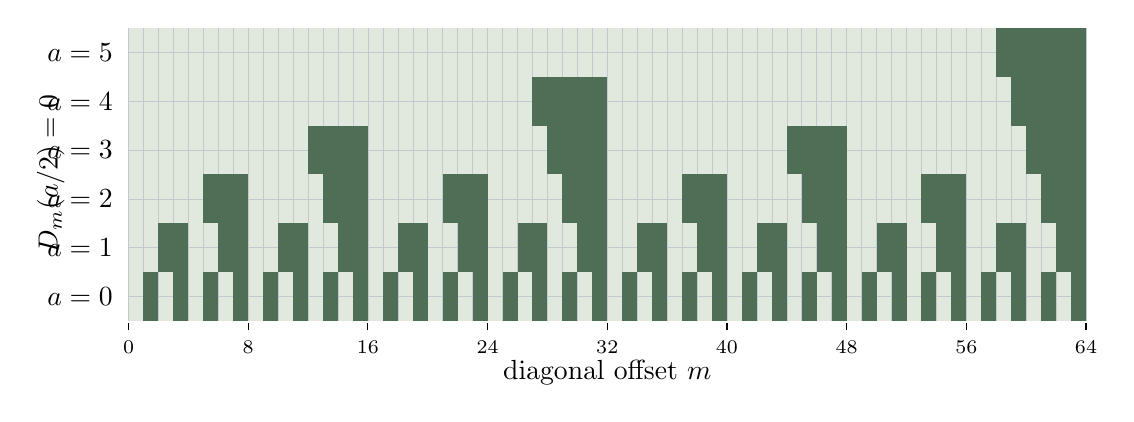
\begin{tikzpicture}[x=0.19cm,y=0.62cm]
  \fill[lightroot] (0,-0.5) rectangle (64,5.5);
  \draw[rulegray,very thin] (0,-0.5) grid[xstep=1,ystep=1] (64,5.5);
  \foreach \q in {0,...,31}{
    \pgfmathtruncatemacro{\m}{2*\q+1}
    \fill[rootcell] (\m, -0.5) rectangle ++(1,1);
  }
  \foreach \q in {0,...,15}{
    \foreach \r in {2,3}{
      \pgfmathtruncatemacro{\m}{4*\q+\r}
      \fill[rootcell] (\m, 0.5) rectangle ++(1,1);
    }
  }
  \foreach \q in {0,...,7}{
    \foreach \r in {5,6,7}{
      \pgfmathtruncatemacro{\m}{8*\q+\r}
      \fill[rootcell] (\m, 1.5) rectangle ++(1,1);
    }
  }
  \foreach \q in {0,...,3}{
    \foreach \r in {12,13,14,15}{
      \pgfmathtruncatemacro{\m}{16*\q+\r}
      \fill[rootcell] (\m, 2.5) rectangle ++(1,1);
    }
  }
  \foreach \q in {0,1}{
    \foreach \r in {27,28,29,30,31}{
      \pgfmathtruncatemacro{\m}{32*\q+\r}
      \fill[rootcell] (\m, 3.5) rectangle ++(1,1);
    }
  }
  \foreach \r in {58,59,60,61,62,63}{
    \fill[rootcell] (\r, 4.5) rectangle ++(1,1);
  }
  \foreach \a in {0,...,5}{
    \node[anchor=east] at (-0.4,\a) {$a=\a$};
  }
  \foreach \m in {0,8,...,64}{
    \draw (\m,-0.55)--(\m,-0.68);
    \node[anchor=north] at (\m,-0.72) {\scriptsize \m};
  }
  \node[rotate=90] at (-5.2,2.5) {$\Diag_m(a/2)=0$};
  \node at (32,-1.55) {diagonal offset $m$};
\end{tikzpicture}
\caption{The exact nonnegative half-integer root raster for
$0\le m<64$ and $0\le a\le5$.  A dark cell means that $2x-a$ divides
$\Diag_m(x)$.  Row $a$ consists of the final $a+1$ residues in each period
$2^{a+1}$.}
\label{fig:root-raster}
\end{figure}

\subsection{Exact values on the negative half-grid}

A negative half-step is finite because it multiplies the generating function
by a polynomial.  Taking $x=-b/2$ in \eqref{eq:D-generating} gives
\begin{equation}
 \sum_{m\ge0}\Diag_m\!\left(-\frac b2\right)z^m
 =(1-z)^b\TM(z^2).
 \label{eq:negative-half-gf}
\end{equation}

\begin{theorem}[Negative half-grid formula]
\label{thm:negative-half}
For $b,m\in\N$,
\begin{equation}
 \boxed{\quad
 \Diag_m\!\left(-\frac b2\right)
 =\sum_{\substack{0\le j\le\min(b,m)\\j\equiv m\ (\mathrm{mod}\ 2)}}
   (-1)^j\binom bj\eps_{(m-j)/2}.
 \quad}
 \label{eq:negative-half-value}
\end{equation}
Consequently, together with \cref{thm:positive-half-roots}, equation
\eqref{eq:negative-half-value} gives a finite exact decision procedure for
every rational root of every $\Diag_m$.
\end{theorem}

\begin{proof}
Expand $(1-z)^b$ and
$\TM(z^2)=\sum_{q\ge0}\eps_qz^{2q}$ in
\eqref{eq:negative-half-gf}.  A term contributes to $z^m$ exactly when
$m-j=2q\ge0$.
\end{proof}

Some low negative arguments simplify sharply.  In the next corollary only,
extend the notation by $\eps_j=0$ for $j<0$.

\begin{corollary}[Selected negative factors]
\label{cor:negative-factors}
For $m\ge0$ and $q\ge1$,
\begin{align}
 \Diag_m\!\left(-\frac12\right)&=\eps_m,
 \label{eq:minus-half}\\
 \Diag_{2q}(-1)&=\eps_q+\eps_{q-1},
 &\Diag_{2q+1}(-1)&=-2\eps_q,
 \label{eq:minus-one}\\
 \Diag_{2q}(-2)&=\eps_q+6\eps_{q-1}+\eps_{q-2},
 &\Diag_{2q+1}(-2)&=-4(\eps_q+\eps_{q-1}).
 \label{eq:minus-two}
\end{align}
In particular,
\begin{align}
 (x+1)\mid\Diag_{2q}(x)
 &\quad\Longleftrightarrow\quad \vtwo(q)\ \text{is even},
 \label{eq:xplus1}\\
 (x+2)\mid\Diag_{2q+1}(x)
 &\quad\Longleftrightarrow\quad \vtwo(q)\ \text{is even}.
 \label{eq:xplus2}
\end{align}
The values $\Diag_{2q+1}(-1)$ and $\Diag_{2q}(-2)$ never vanish.
\end{corollary}

\begin{proof}
Equation \eqref{eq:minus-half} follows because
$(1-z)\TM(z^2)=\TM(z)$.  Equations \eqref{eq:minus-one} and
\eqref{eq:minus-two} follow by multiplying $\TM(z^2)$ by
$(1-z)^2$ and $(1-z)^4$.

When $q\ge1$, passing from $q-1$ to $q$ changes the binary digit sum by
$1-\vtwo(q)$.  Hence
$\eps_q=-\eps_{q-1}$ exactly when $\vtwo(q)$ is even.  This proves the two
factor criteria.  Finally, the middle term in
$\eps_q+6\eps_{q-1}+\eps_{q-2}$ has magnitude six while the other two have
total magnitude at most two.
\end{proof}

The first two strict negative half-integers are also never roots:
$\Diag_m(-1/2)=\eps_m\ne0$, and
\[
 \Diag_m(-3/2)=\eps_m-2\eps_{m-1}+\eps_{m-2}\ne0.
\]
For $m\ge2$, the second assertion would require three consecutive
Thue--Morse signs to be equal, while every three consecutive positions
contain an aligned pair $(2q,2q+1)$ of opposite signs.  The cases $m=0,1$
are immediate from the same formula with the zero extension just stated.

The experiments included with this article suggest a stronger statement.

\begin{conjecture}[No strict negative half-integer roots]
\label{conj:no-negative-strict-half}
For all $m,r\in\N$,
\begin{equation}
 \Diag_m\!\left(-r-\frac12\right)\ne0.
 \label{eq:no-negative-strict-half}
\end{equation}
Equivalently, every negative rational root of $\Diag_m$ is an integer.
\end{conjecture}

The accompanying exact Python program found no counterexample for every odd
$1\le b\le63$ and every $0\le m\le10000$ in
$\Diag_m(-b/2)$.  This finite computation is evidence only; the conjecture is
not used elsewhere.  Formula \eqref{eq:negative-half-value} converts the
problem into a nonvanishing statement for parity-restricted binomial sums of
consecutive Thue--Morse signs.

\section{Fast exact evaluation}
\label{sec:algorithms}

There are three distinct computational tasks, and they should not be confused:
\begin{enumerate}
 \item generate the symbolic polynomial $\Diag_m(x)$ for a fixed diagonal;
 \item evaluate one near-edge value $\Diag_m(n)$ when $m$ is moderate;
 \item evaluate an arbitrary table entry when $m=k-n-1$ may be enormous.
\end{enumerate}
The best formula is different in each regime.

\subsection{Symbolic generation of any diagonal}

For a single symbolic polynomial, \eqref{eq:D-rising} is direct and finite.
The following Wolfram Language definition automatically replaces all manually
entered diagonal rules:

\begin{lstlisting}[style=code,language=Wolfram]
tmSign[q_Integer?NonNegative] := (-1)^ThueMorse[q];

risingTwoX[x_, 0] := 1;
risingTwoX[x_, p_Integer?Positive] :=
  Product[2 x + j, {j, 0, p - 1}];

DiagonalPolynomial[m_Integer?NonNegative, x_] := Expand @ Sum[
  With[{p = m - 2 q}, tmSign[q] risingTwoX[x, p]/p!],
  {q, 0, Floor[m/2]}
];
\end{lstlisting}

For example,
\begin{lstlisting}[style=code,language=Wolfram]
Table[Factor[DiagonalPolynomial[m, x]], {m, 0, 20}]
\end{lstlisting}
generates the first twenty-one diagonal laws exactly.  No calls to
\texttt{InterpolatingPolynomial}, numerical fitting, or rational
reconstruction are involved.

When a whole prefix $\Diag_0,\ldots,\Diag_M$ is needed, the Newton recurrence
\eqref{eq:newton} reuses previous work:

\begin{lstlisting}[style=code,language=Wolfram]
lambda[r_Integer?Positive, x_] :=
  2 x + 2 - 2^(IntegerExponent[r, 2] + 1);

diagonalFormal[0] = 1;
diagonalFormal[m_Integer?Positive] := diagonalFormal[m] = Expand[
  Sum[lambda[r, formalX] diagonalFormal[m - r], {r, 1, m}]/m
];
\end{lstlisting}

The two generators are algebraically independent implementations and are
therefore useful for regression testing each other.

\subsection{Direct exact evaluation}

At an integer row $n$, the finite binomial formula is
\begin{equation}
 \Diag_m(n)=\sum_{q=0}^{\lfloor m/2\rfloor}
 \eps_q\binom{2n+m-2q-1}{m-2q}.
 \label{eq:direct-integer-value}
\end{equation}
For a small or moderate $m$ this is excellent: it has only
$\lfloor m/2\rfloor+1$ exact summands.  The corresponding Wolfram Language
routine is

\begin{lstlisting}[style=code,language=Wolfram]
DiagonalValue[m_Integer?NonNegative, n_Integer?NonNegative] := Sum[
  With[{p = m - 2 q},
    tmSign[q] Binomial[2 n + p - 1, p]
  ],
  {q, 0, Floor[m/2]}
];
\end{lstlisting}

The block law \eqref{eq:D-block-row} first reduces an arbitrary $m$ modulo
$B=2^{2n+1}$:
\begin{equation}
 \Diag_m(n)=\eps_{\lfloor m/B\rfloor}\Diag_{m\bmod B}(n).
 \label{eq:diagonal-block-reduction}
\end{equation}
Unlike the original code's block rule, this version acts directly on the
natural diagonal offset.  It avoids bookkeeping caused by the shift $n+1$.

\subsection{Logarithmic-time signed prefix moments}

The direct sum is still unsuitable when the reduced offset is very large.
The key observation is that, for fixed $n\ge1$, its binomial kernel is a
polynomial of degree $2n-1$ in the Thue--Morse index $q$:
\begin{equation}
 \binom{2n+m-2q-1}{m-2q}
 =\binom{2n+m-2q-1}{2n-1}
 =\sum_{d=0}^{2n-1}c_d(m,n)q^d.
 \label{eq:kernel-polynomial}
\end{equation}
Thus only finitely many signed prefix moments are required.

\begin{definition}[Signed Thue--Morse prefix moments]
For $N,d\in\N$, let
\begin{equation}
 M_d(N)=\sum_{q=0}^{N-1}\eps_qq^d.
 \label{eq:prefix-moment}
\end{equation}
The sum is exclusive at $N$; $M_d(0)=0$.
\end{definition}

\begin{theorem}[Binary divide-and-conquer recurrence]
\label{thm:moment-recurrence}
For $N,d\in\N$,
\begin{align}
 M_d(2N)
 &=-\sum_{j=0}^{d-1}\binom dj2^jM_j(N),
 \label{eq:moment-even}\\
 M_d(2N+1)
 &=M_d(2N)+\eps_N(2N)^d.
 \label{eq:moment-odd}
\end{align}
The sum in \eqref{eq:moment-even} is empty when $d=0$.
\end{theorem}

\begin{proof}
Pair the terms with indices $2q$ and $2q+1$ and use
\eqref{eq:tm-doubling}:
\begin{align*}
 M_d(2N)
 &=\sum_{q=0}^{N-1}
   \left(\eps_{2q}(2q)^d+\eps_{2q+1}(2q+1)^d\right)\\
 &=\sum_{q=0}^{N-1}\eps_q\left((2q)^d-(2q+1)^d\right)\\
 &=-\sum_{j=0}^{d-1}\binom dj2^j
     \sum_{q=0}^{N-1}\eps_qq^j.
\end{align*}
The highest-degree terms cancel.  Adding the final term at index $2N$ gives
\eqref{eq:moment-odd}.
\end{proof}

Let $L=\lfloor m/2\rfloor+1$.  Combining
\eqref{eq:kernel-polynomial} with \eqref{eq:prefix-moment} gives
\begin{equation}
 \boxed{\quad
 \Diag_m(n)=\sum_{d=0}^{2n-1}c_d(m,n)M_d(L)
 \qquad(n\ge1).
 \quad}
 \label{eq:moment-evaluator}
\end{equation}
The recursion depth for $M_d(L)$ is $O(\log L)$.  At each level, computing
all moments through degree $2n-1$ by \eqref{eq:moment-even} uses
$O(n^2)$ arithmetic operations.  Ignoring integer multiplication bit costs,
the evaluator therefore uses
\begin{equation}
 O(n^2\log m)
 \label{eq:moment-complexity}
\end{equation}
exact arithmetic operations, rather than $O(m)$ summands.

\begin{algorithm}[Hybrid evaluator]
\label{alg:hybrid}
Given $n,k\in\N$:
\begin{enumerate}
 \item If $k\le n$, return $0$.
 \item Set $m=k-n-1$, $B=2^{2n+1}$, and write $m=qB+r$.
 \item Compute the core value $\Diag_r(n)$ by the direct sum if $r$ is below
       a chosen small cutoff; otherwise use \eqref{eq:moment-evaluator}.
 \item Return $\eps_q\Diag_r(n)$.
\end{enumerate}
\end{algorithm}

The cutoff only chooses between two exact algorithms; it does not affect the
result.  The supplied implementation uses $128$ by default.

\begin{lstlisting}[style=code,language=Wolfram]
tmPrefixMoments[0, maxDegree_Integer?NonNegative] :=
  ConstantArray[0, maxDegree + 1];

tmPrefixMoments[length_Integer?Positive, maxDegree_Integer?NonNegative] :=
  tmPrefixMoments[length, maxDegree] = Module[
    {half = Quotient[length, 2], lower, paired},
    lower = tmPrefixMoments[half, maxDegree];
    paired = Table[
      If[d == 0, 0,
        -Sum[Binomial[d, j] 2^j lower[[j + 1]], {j, 0, d - 1}]
      ],
      {d, 0, maxDegree}
    ];
    If[OddQ[length],
      paired += tmSign[half] Table[(2 half)^d, {d, 0, maxDegree}]
    ];
    paired
  ];
\end{lstlisting}

For $n\ge1$, the polynomial coefficients $c_d(m,n)$ are obtained exactly
from
\[
 \frac{1}{(2n-1)!}\prod_{j=1}^{2n-1}(m-2q+j).
\]
The full source file \texttt{diagonal\_polynomials.wl} contains this
contraction, block reduction, a compact replacement for the original
\texttt{s}, and a literal repeated-prefix reference implementation.

\subsection{Memory and implementation notes}

The memoized moment routine stores vectors keyed by the pair
$(N,d_{\max})$.  A single query touches only the binary ancestors
$N,\lfloor N/2\rfloor,\lfloor N/4\rfloor,\ldots$, so its live recursion
depth is logarithmic.  For a long batch with many unrelated degree bounds,
one may remove memoization or cache moments at a fixed maximum degree and
truncate as needed.

Exact integer sizes can be very large.  Complexity
\eqref{eq:moment-complexity} counts arithmetic operations, not bit
operations; this is the appropriate distinction because the output itself
may contain thousands or millions of bits.  The algorithm avoids artificial
work proportional to the index $m$, but it cannot avoid the cost of storing
the exact answer.

The local recurrence \eqref{eq:local-pde} remains preferable when a dense
rectangular region is desired.  The moment method is designed for sparse
random access to isolated entries.  The diagonal polynomial and Newton--Bell
methods are designed for symbolic dependence on $n$.  Keeping these use cases
separate leads to simpler and faster code.

\section{Connection with the Fabius and Rvachev approximation layer}
\label{sec:fabius}

The diagonal theory is purely discrete, but it lands exactly on the finite
polynomials used in the repository's Fabius--Rvachev approximants.  The Lean
formalization proves that the order-$k$ iterated prefix coefficients below the
first dyadic cutoff are the coefficients of the approximation polynomial
$p_{k-1}$, and that division by
$2^{\binom{k-1}{2}}$ gives the corresponding step-approximant values at cell
centers \cite{proveit-approx}.

For the odd order $k=2n+1$ considered here, the finite approximation
polynomial is precisely
\begin{equation}
 p_{2n}(z)=H_{2n}(z)
 =\prod_{j=1}^{2n}(1+z+\cdots+z^{2^j-1}).
 \label{eq:p-H}
\end{equation}
Therefore, whenever $0\le m<2^{2n+1}$,
\begin{equation}
 \Diag_m(n)=[z^m]p_{2n}(z),
 \label{eq:D-approx-coeff}
\end{equation}
and the normalized step height is
\begin{equation}
 \frac{\Diag_m(n)}{2^{\binom{2n}{2}}}.
 \label{eq:normalized-edge}
\end{equation}
The normalizing denominator is exactly the plateau height $C$ in
\eqref{eq:row-constants}.  Thus the complement law
\eqref{eq:core-complement} becomes a normalized reflection around $1/2$,
and the central plateau \eqref{eq:core-plateau} becomes the level $1$.

For a fixed diagonal offset $m$, combine \eqref{eq:D-large-n} with
$C=2^{n(2n-1)}$ to obtain
\begin{equation}
 \frac{\Diag_m(n)}{2^{\binom{2n}{2}}}
 =\frac{2^mn^m}{m!}\,2^{-n(2n-1)}
 \left(1+\frac{m(m-1)}{4n}+\bigO(n^{-2})\right).
 \label{eq:normalized-diagonal-asymptotic}
\end{equation}
Hence every fixed number of coefficient cells from the left edge is
suppressed by a quadratic exponential in $n$, up to a polynomial factor.
This is an exact quantitative boundary-layer statement for the finite
approximants.  It is consistent with the infinite-order flatness of the
limiting Fabius/Rvachev functions, but it should not be confused with an
asymptotic at a fixed spatial argument: the cell represented by a fixed $m$
moves toward the support endpoint as the grid is refined.

The block factorization also clarifies why the early repeated-summation
picture sees the Fabius shape at all.  After division by $H_{2n}(1)$, the coefficients of $H_{2n}$ are the
probability mass function of a sum of independent discrete uniforms on
$\{0,\ldots,2^j-1\}$, while the normalized limit is related to the continuous
sum of geometrically scaled uniforms appearing in the probability model of
Rvachev's up-function.  The present article does not reprove that analytic
limit; it isolates the exact finite coefficient algebra on which that limit
acts.

\section{Further deductions and research directions}
\label{sec:future}

The closed form \eqref{eq:D-rising} resolves the basic diagonal question, but
it also exposes several directions that are not visible from the first eight
polynomials.

\subsection{Scaling regimes beyond fixed diagonals}

The fixed-$m$ asymptotic \eqref{eq:D-large-n} is only the extreme left edge.
There are at least four natural regimes for $m=m(n)$:
\begin{enumerate}
 \item $m$ fixed;
 \item $m\to\infty$ but $m=o(2^n)$, where only the first few geometric upper
       bounds in \eqref{eq:restricted-compositions} are active;
 \item $m$ proportional to the standard deviation of the restricted-uniform
       sum, where a local central limit theorem should control $h_{2n,m}$;
 \item $m$ within $O(n)$ of the exact plateau and zero-run boundaries, where
       finite edge corrections dominate.
\end{enumerate}
A uniform saddle-point analysis of
$H_{2n}(z)$ could connect the polynomial edge law to the Gaussian bulk and
the exact flat plateau without passing through separate approximations.

\subsection{Residual factors and zero geometry}

After removing the completely classified nonnegative rational factor
$R_m^+$ and the negative integer factors detected by
\eqref{eq:negative-half-value}, the remaining factor often appears
irreducible over $\Q$ in low degrees.  Questions include:
\begin{itemize}
 \item Are all nonnegative half-integer zeros simple?
 \item Can the negative integer roots be characterized by binary automata in
       the pair $(m,r)$ from the binomial sums at $x=-r$?
 \item Does \cref{conj:no-negative-strict-half} hold?
 \item What is the limiting distribution of the nonrational complex zeros of
       $\Diag_m$ after an $m$-dependent scaling?
\end{itemize}
The half-step lowering law suggests that finite-difference analogues of
classical results on Appell and Sheffer zero interlacing may be relevant, but
$\TM(z^2)$ is not a positivity-preserving prefactor, so standard real-rooted
arguments do not apply directly.

\subsection{Automatic and \texorpdfstring{$p$-adic}{p-adic} structure}

The cumulants \eqref{eq:lambda} depend on $r$ only through $\vtwo(r)$.  This
makes the Newton recurrence an unusual hybrid of Bell-polynomial and
automatic-sequence structure.  It is natural to ask for:
\begin{itemize}
 \item finite automata or linear representations for coefficient residues of
       the primitive polynomials $Q_m$ modulo odd primes;
 \item exact Newton polygons of $Q_m$ at $2$ beyond the coarse bound
       \eqref{eq:coefficient-v2-bound};
 \item analogues for generalized base-$b$ Thue--Morse products
       $\prod_{j\ge0}(1-z^{b^j})$ or for weighted digit characters.
\end{itemize}
For a general digit character, the logarithmic cumulants are controlled by
$b$-adic divisibility, so much of the Riordan and Bell machinery survives
with $\vtwo$ replaced by $\nu_b$ and with a different finite block.

\subsection{Formalization opportunities}

The repository already formalizes the inclusive-prefix convolution, dyadic
zero runs, finite approximation polynomials, and corrected normalization.
The following additions are comparatively self-contained candidates for Lean
formalization:
\begin{enumerate}
 \item the shifted-table identity \eqref{eq:s-prefix-identification};
 \item the diagonal generating function \eqref{eq:D-generating} and finite
       formula \eqref{eq:D-rising};
 \item the half-step recurrence \eqref{eq:half-step};
 \item the finite-block theorem \eqref{eq:half-block-factorization};
 \item primitive normalization and the exact denominator theorem;
 \item the rational-root restriction;
 \item the signed-prefix-moment recurrences and correctness of the fast
       evaluator.
\end{enumerate}
Most proofs are finite formal-power-series or elementary integer-divisibility
arguments and should integrate naturally with the existing modules on
Thue--Morse generating series and Prouhet cancellation.

\section{Summary of the main formulas}
\label{sec:summary}

For quick reference, the complete computational chain is:
\begin{align*}
 \eps_q&=(-1)^{\bitsum(q)},\\
 \TM(z)&=\sum_{q\ge0}\eps_qz^q
          =\prod_{j\ge0}(1-z^{2^j}),\\
 s(n,k)&=0\quad(k\le n),\\
 s(n,k)&=\Diag_{k-n-1}(n)\quad(k>n),\\
 \sum_{m\ge0}\Diag_m(x)z^m
 &=\frac{\TM(z^2)}{(1-z)^{2x}},\\
 \Diag_m(x)&=\sum_{q=0}^{\lfloor m/2\rfloor}
 \eps_q\frac{\rising{(2x)}{m-2q}}{(m-2q)!},\\
 m\Diag_m(x)
 &=\sum_{r=1}^{m}
   \left(2x+2-2^{\vtwo(r)+1}\right)\Diag_{m-r}(x),\\
 \Diag_m(x)-\Diag_m(x-\tfrac12)&=\Diag_{m-1}(x),\\
 Q_m(x)&=\frac{m!}{2^{\lceil m/2\rceil}}\Diag_m(x)\in\Z[x]
 \quad\text{and is primitive},\\
 \operatorname{den}(\Diag_m)&=
 \frac{m!}{2^{\min(\vtwo(m!),\lceil m/2\rceil)}}.
\end{align*}
For $a\ge0$, with $B_a=2^{a+1}$,
\[
 \Diag_m(a/2)=0
 \quad\Longleftrightarrow\quad
 m\bmod B_a\ge B_a-a-1.
\]
For $b\ge0$,
\[
 \Diag_m(-b/2)=
 \sum_{\substack{0\le j\le\min(b,m)\\j\equiv m\ (2)}}
 (-1)^j\binom bj\eps_{(m-j)/2}.
\]
For arbitrary random access, expand
$\binom{2n+m-2q-1}{2n-1}$ as a degree-$(2n-1)$ polynomial in $q$ and contract
it with the recursively computed signed moments $M_d(\lfloor m/2\rfloor+1)$.
This completes the passage from a finite list of hand-entered diagonal rules
to a general symbolic and algorithmic theory.

\appendix

\section{Nonnegative rational factors through \texorpdfstring{$m=31$}{m=31}}
\label{app:factor-table}

The following table lists $\mathcal A_m$ from \eqref{eq:Am}.  The displayed
squarefree product $\prod_{a\in\mathcal A_m}(2x-a)$ contains one copy of every
nonnegative rational linear factor; an empty set means that $\Diag_m$ has no
nonnegative rational zero.

\begin{center}
\small
\begin{longtable}{r@{\quad}l|r@{\quad}l}
\toprule
$m$ & $\mathcal A_m$ & $m$ & $\mathcal A_m$\\
\midrule
\endfirsthead
\toprule
$m$ & $\mathcal A_m$ & $m$ & $\mathcal A_m$\\
\midrule
\endhead
0&$\varnothing$&16&$\varnothing$\\
1&$\{0\}$&17&$\{0\}$\\
2&$\{1\}$&18&$\{1\}$\\
3&$\{0,1\}$&19&$\{0,1\}$\\
4&$\varnothing$&20&$\varnothing$\\
5&$\{0,2\}$&21&$\{0,2\}$\\
6&$\{1,2\}$&22&$\{1,2\}$\\
7&$\{0,1,2\}$&23&$\{0,1,2\}$\\
8&$\varnothing$&24&$\varnothing$\\
9&$\{0\}$&25&$\{0\}$\\
10&$\{1\}$&26&$\{1\}$\\
11&$\{0,1\}$&27&$\{0,1,4\}$\\
12&$\{3\}$&28&$\{3,4\}$\\
13&$\{0,2,3\}$&29&$\{0,2,3,4\}$\\
14&$\{1,2,3\}$&30&$\{1,2,3,4\}$\\
15&$\{0,1,2,3\}$&31&$\{0,1,2,3,4\}$\\
\bottomrule
\end{longtable}
\end{center}

The table makes the nested terminal windows before powers of two visible.  At
$m=2^{a+1}-a-1,\ldots,2^{a+1}-1$, the new root $x=a/2$ appears; lower-period
root patterns continue independently underneath it.

\section{Complete Wolfram Language source}
\label{app:wolfram}

The following listing is the exact source distributed as
\texttt{diagonal\_polynomials.wl}.

\lstinputlisting[style=code,language=Wolfram,basicstyle=\ttfamily\scriptsize]{diagonal_polynomials.wl}

\section{Complete Python verification source}
\label{app:python}

The Python program uses SymPy exact arithmetic.  It verifies the direct and
Newton--Bell polynomial generators, the half-step law, literal repeated
prefix summation, finite-block reduction, prefix-moment evaluation, primitive
normalization, exact denominators, and both half-grid formulas.  It also
contains the finite scan reported after
\cref{conj:no-negative-strict-half}.

\lstinputlisting[style=code,language=Python,basicstyle=\ttfamily\scriptsize]{diagonal_polynomials.py}

\section{Reproduction commands}
\label{app:reproduce}

From the directory containing the source files:

\begin{lstlisting}[style=code]
python diagonal_polynomials.py --max-degree 12 --verify
python diagonal_polynomials.py --max-degree 3 --scan-negative-half
latexmk -pdf -interaction=nonstopmode -halt-on-error \
  thue_morse_diagonal_polynomials.tex
\end{lstlisting}

The first command performs the theorem-level regression checks and prints
factored polynomials.  The second performs the exact finite conjecture scan
through odd $b\le63$ and $m\le10000$.  The LaTeX source uses only files
included in the archive.

\begin{thebibliography}{99}

\bibitem{allouche-shallit-1999}
J.-P. Allouche and J. Shallit,
\newblock The ubiquitous Prouhet--Thue--Morse sequence,
\newblock in \emph{Sequences and Their Applications: Proceedings of SETA '98},
C. Ding, T. Helleseth, and H. Niederreiter, eds.,
Springer Series in Discrete Mathematics and Theoretical Computer Science,
Springer, London, 1999, pp. 1--16.

\bibitem{automatic-sequences}
J.-P. Allouche and J. Shallit,
\newblock \emph{Automatic Sequences: Theory, Applications, Generalizations},
\newblock Cambridge University Press, Cambridge, 2003.

\bibitem{comtet}
L. Comtet,
\newblock \emph{Advanced Combinatorics: The Art of Finite and Infinite
Expansions},
\newblock D. Reidel, Dordrecht, 1974.

\bibitem{riordan-group}
L. W. Shapiro, S. Getu, W.-J. Woan, and L. C. Woodson,
\newblock The Riordan group,
\newblock \emph{Discrete Applied Mathematics} \textbf{34} (1991), 229--239,
\newblock \url{https://doi.org/10.1016/0166-218X(91)90088-E}.

\bibitem{sprugnoli}
R. Sprugnoli,
\newblock Riordan arrays and combinatorial sums,
\newblock \emph{Discrete Mathematics} \textbf{132} (1994), 267--290.

\bibitem{roman-umbral}
S. Roman,
\newblock \emph{The Umbral Calculus},
\newblock Pure and Applied Mathematics, vol. 111, Academic Press, New York,
1984.

\bibitem{proveit-early}
V. Reshetnikov,
\newblock \emph{$K$-fold summation over the signed Thue--Morse sequence},
\newblock early research note in the \texttt{ProveIt} repository,
\path{Analysis/FabiusFunction/docs/archive/early-notes/},
file object \texttt{837bdf2b6711388b83d2e65c92824aa1f3e4c48d},
accessed 3 September 2026.

\bibitem{proveit-prefix}
V. Reshetnikov,
\newblock \texttt{FabiusFunction/ThueMorsePrefix.lean},
\newblock formal development of inclusive iterated prefixes, convolution, and
zero runs in the \texttt{ProveIt} repository,
file object \texttt{1c6fe79e3a71fb2f06efd6817aa497aa9aa3753e},
accessed 3 September 2026.

\bibitem{proveit-approx}
V. Reshetnikov,
\newblock \texttt{FabiusFunction/ThueMorseApproximation.lean},
\newblock formal development of finite approximation polynomials, corrected
normalization, and step approximants in the \texttt{ProveIt} repository,
file object \texttt{5678201a0060b9cf91ef3fb2995c647b73b5f423},
accessed 3 September 2026.

\bibitem{proveit-audit}
V. Reshetnikov,
\newblock \texttt{FabiusFunction/DraftCounterexamples.lean},
\newblock machine-checked audit of false proxy, normalization, and error
claims in an early draft, in the \texttt{ProveIt} repository,
file object \texttt{6de3948507c382c95521f6de768bc43ba7a8081f},
accessed 3 September 2026.

\end{thebibliography}

\end{document}
